\subsubsection{x86: 3 Argumente}
% to be sync: \subsubsection{x86: 3 integer arguments}

\myparagraph{MSVC}

Beim Kompilieren mit MSVC 2010 Express wird folgende Ausgabe erzeugt:

\begin{lstlisting}[style=customasmx86]
$SG3830	DB	'a=%d; b=%d; c=%d', 00H

...

	push	3
	push	2
	push	1
	push	OFFSET $SG3830
	call	_printf
	add	esp, 16					; 00000010H
\end{lstlisting}

Fast die gleiche Ausgabe, allerdings sind jetzt die \printf-Argumente in umgekehrter Reihenfolge
auf dem Stack hinterlegt. Das erste Argument kommt zuerst.

Die Variablen vom Typ \Tint sind in einer 32-Bit-Umgebung 32 Bit breit, was 4 Byte entspricht.

In diesem Fall sind 4 Argumente vorhanden. $4*4 = 16$~---diese benötigen exakt 16 Byte auf dem Stack
einen 32-Bit-Zeiger auf eine Zeichenkette und 3 Zahlen des Typs \Tint.

\myindex{x86!\Instructions!ADD}
\myindex{x86!\Registers!ESP}
\myindex{cdecl}
Wenn der \gls{stack pointer} (\ESP-Register) nach einem Funktionsaufruf durch die Anweisung
\INS{ADD ESP, X} wiederhergestellt wird, wird die Anzahl Argumente oft einfach durch
die Division von X durch 4 abgeleitet.

Natürlich ist dies eine Eigenheit der \emph{cdecl}-Aufrufkonvention und nur für 32-Bit-Umgebungen gültig
(siehe auch Abschnitt über Aufrufkonventionen~(\myref{sec:callingconventions})).

In bestimmten Fällen in denen mehrere Funktionen direkt hintereinander beendet werden, kann
der Compiler mehrere \q{ADD ESP, X}-Anweisungen in einer zusammenfassen:

\begin{lstlisting}[style=customasmx86]
push a1
push a2
call ...
...
push a1
call ...
...
push a1
push a2
push a3
call ...
add esp, 24
\end{lstlisting}

Hier ist ein Beispiel aus einer realen Applikation:

\lstinputlisting[caption=x86,style=customasmx86]{patterns/03_printf/x86/add_example_DE.lst}

\clearpage
\myparagraph{MSVC und \olly}
\myindex{\olly}

% TODO User-Land is not the correct term...
Sehen wir uns das Beispiel in \olly an, der einer der populärsten User-Land-Win32-Debugger ist.
Wenn das Beispiel in MSVC 2012 mit der Option \GTT{/MD} kompiliert wird, wird gegen \GTT{MSVCR*.DLL} gelinkt.
Somit kann die importierte Funktion klar im Debugger gesehen werden.

Anschließend wird die ausführbare Datei in \olly geladen.
Der erste Breakpoint ist in \GTT{ntdll.dll}, F9 startet die Ausführung.
Der zweite Breakpoint ist im \ac{CRT}-Code.

Jetzt muss die \main-Funktion gefunden werden, die sich ganz oben im Code befindet
(MSVC allokiert die \main-Funktion ganz zu Beginn der Code-Sektion): 
\begin{figure}[H]
\centering
\myincludegraphics{patterns/03_printf/x86/olly3_1.png}
\caption{\olly: Der Start der \main-Funktion}
\label{fig:printf3_olly_1}
\end{figure}

Um den \ac{CRT}-Code zu überspringen (der hier nicht von Interesse ist) müssen
folgende Schritte ausgeführt werden: Klicken auf die \INS{PUSH EBP}-Anweisung,
Drücken von F2 (Breakpoint setzen) und Drücken von F9 (Starten

\clearpage
Sechsmaliges Drücken von F8 (\stepover) überspringt sechs Anweisungen:

\begin{figure}[H]
\centering
\myincludegraphics{patterns/03_printf/x86/olly3_2.png}
\caption{\olly: vor der Ausführung von\printf}
\label{fig:printf3_olly_2}
\end{figure}

Jetzt zeigt der \ac{PC} auf die \INS{CALL printf}-Anweisung.
\olly hebt, wie andere Debugger auch, den Wert des Registers hervor, welches sich geändert hat.
Bei jedem Drücken von F8 ändert sich also \EIP und der Wert wird in rot angezeigt.
\ESP ändert sich ebenfalls, weil die Werte der Argumente auf dem Stack gesichert werden.\\
\\
Wo befinden sich die Werte auf dem Stack? Ein Blick auf das untere, rechte Fenster
des Debuggers liefert die Antwort:

\begin{figure}[H]
\centering
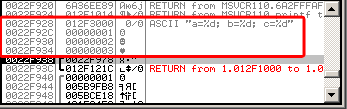
\includegraphics[width=0.5\textwidth]{patterns/03_printf/x86/olly3_stack.png}

\caption{\olly: Stack nachdem der Wert des Arguments gesichert wurde (Das rote Rechteck wurde vom Autor hinzugefügt)}
\end{figure}

Es sind hier drei Spalten sichtbar: Die Adresse im Stack, der Wert im Stack und einige weitere \olly-Kommentare.
\olly versteht \printf{}-ähnliche Zeichenketten und zeigt sie zusammen mit den drei \emph{angehangenen} Werten an.
% to be sync: \olly can detect pointers to ASCII strings in stack, so it reports the \printf{}-string here.

Es ist möglich einen Rechtsklick auf den Formatstring und anschließend auf \q{Follow in dump} zu klicken.
Der Formatstring wird in dem linken-unterem Debugger erscheinen, welches immer einen Teil des Speichers zeigt.
Diese Speicherwerte können editiert werden.
Es ist möglich den Formatstring zu verändern, was die Ausgabe dieses Beispiels ebenfalls verändern würde.
In diesem Fall ist das nicht sehr nützlich, aber es könnte eine gute Übung sein um ein Gefühl dafür zu
bekommen wie hier alles funktioniert.

\clearpage
Drücken von F8 (\stepover).

Es erscheint die folgende Ausgabe auf der Konsole:

\lstinputlisting{patterns/03_printf/x86/console.txt}

Nachfolgend die Änderungen in den Registern und der Status des Stacks:

\begin{figure}[H]
\centering
\myincludegraphics{patterns/03_printf/x86/olly3_3.png}
\caption{\olly nach der Ausfühung von \printf{}}
\label{fig:printf3_olly_3}
\end{figure}

Das Register \EAX enthält nun \GTT{0xD} (13).
Dies ist auch richtig, weil \printf die Anzahl der ausgegeben Zeichen zurück gibt.
Der Wert von \EIP hat sich verändert: er enthält nun die Adresse der Anweisung, die
nach \INS{CALL printf} kommt.
Die Werte von \ECX und \EDX haben sich ebenfalls geändert.
Offensichtlich nutzt die \printf-Funktion diese für interne Zwecke.

Ein wichtiger Punkt ist, dass weder der \ESP-Wert, noch der Status des Stacks sich geändert haben!
Es ist klar erkennbar, dass der Formatstring und die drei entsprechenden Werte immer noch da sind.
Dies ist das Verhalten der \emph{cdecl}-Aufrufkonvention: \gls{callee} setzt \ESP nicht auf den vorherigen
Wert zurück. Dies ist die Aufgabe der \gls{caller}.

\clearpage
Durch erneutes Drücken von F8 wird die Anweisung \INS{ADD ESP, 10} ausgeführt:

\begin{figure}[H]
\centering
\myincludegraphics{patterns/03_printf/x86/olly3_4.png}
\caption{\olly: Nach der Ausführung von \INS{ADD ESP, 10}}
\label{fig:printf3_olly_4}
\end{figure}

\ESP hat sich geändert, aber die Werte sind immer noch auf dem Stack!
Das liegt natürlich daran, dass es keine Notwendigkeit gibt diese Werte auf Null zu setzen oder Ähnliches.
Alle oberhalb des Stack-Pointers (\ac{SP}) ist \emph{Rauschen} oder \emph{\garbage{}} und hat keine Bedeutung.
Es wäre zeitintensiv und unnötig die ungenutzten Stack-Einträge zurück zu setzen.

\myparagraph{GCC}

Nun wird das gleiche Programm unter Linux mit GCC 4.4.1 kompiliert und in \IDA untersucht:

\lstinputlisting[style=customasmx86]{patterns/03_printf/x86/x86_1.asm}

Es ist erkennbar, dass der Unterschied zwischen MSVC- und GCC-Code lediglich die Art ist,
auf der die Argumente auf dem Stack gespeichert werden.
Hier arbeitet GCC direkt mit dem Stack ohne Benutzung von \PUSH/\POP.

\myparagraph{GCC und GDB}
\myindex{GDB}

Nachfolgend das Beispiel mit \ac{GDB} unter Linux.

Die Option \GTT{-g} weist den Compiler an, Debugging-Informationen in die ausführbare Datei einzufügen.

\begin{lstlisting}
$ gcc 1.c -g -o 1
\end{lstlisting}

\begin{lstlisting}
$ gdb 1
GNU gdb (GDB) 7.6.1-ubuntu
...
Reading symbols from /home/dennis/polygon/1...done.
\end{lstlisting}

\begin{lstlisting}[caption=Setzen eines Breakpoints auf \printf]
(gdb) b printf
Breakpoint 1 at 0x80482f0
\end{lstlisting}

Ausführen.
Im Quellcode ist keine \printf-Funktion, also kann \ac{GDB} sie nicht anzeigen.

\begin{lstlisting}
(gdb) run
Starting program: /home/dennis/polygon/1 

Breakpoint 1, __printf (format=0x80484f0 "a=%d; b=%d; c=%d") at printf.c:29
29	printf.c: No such file or directory.
\end{lstlisting}

Ausgeben von 10 Stack-Einträgen. Die Spalte ganz links enthält die Adressen auf dem Stack.

\begin{lstlisting}
(gdb) x/10w $esp
0xbffff11c:	0x0804844a	0x080484f0	0x00000001	0x00000002
0xbffff12c:	0x00000003	0x08048460	0x00000000	0x00000000
0xbffff13c:	0xb7e29905	0x00000001
\end{lstlisting}

Das allererste Element ist \ac{RA} (\GTT{0x0804844a}).
Dies kann durch das Disassemblieren des Speichers an dieser Stelle überprüft werden:

\begin{lstlisting}[label=NOP_as_XCHG_example,style=customasmx86]
(gdb) x/5i 0x0804844a
   0x804844a <main+45>:	mov    $0x0,%eax
   0x804844f <main+50>:	leave  
   0x8048450 <main+51>:	ret    
   0x8048451:	xchg   %ax,%ax
   0x8048453:	xchg   %ax,%ax
\end{lstlisting}

Die beiden \INS{XCHG}-Anweisungen sind Idle-Anweisungen, analog zu \ac{NOP}.

Das zweite Element (\GTT{0x080484f0}) ist die Adresse des Formatstrings:

\begin{lstlisting}
(gdb) x/s 0x080484f0
0x80484f0:	"a=%d; b=%d; c=%d"
\end{lstlisting}

Die nächsten drei Elemente (1, 2, 3) sind die \printf-Argumente.
Der Rest der Elemente kann lediglich \q{garbage} auf dem Stack sein,
oder auch Werte von anderen Funktionen, deren lokale Variablen usw.
An dieser Stelle können sie ignoriert werden.

Ausführen von \q{finish}.
Dieses Kommando führt dazu, dass GDB \q{alle Anweisungen bis zum Ende der Funktion ausführt}.
In diesem Fall: Ausführen bis zum Ende von \printf.

\begin{lstlisting}
(gdb) finish
Run till exit from #0  __printf (format=0x80484f0 "a=%d; b=%d; c=%d") at printf.c:29
main () at 1.c:6
6		return 0;
Value returned is $2 = 13
\end{lstlisting}

\ac{GDB} zeigt was \printf in \EAX zurück gibt (13).
Die ist die Anzahl der ausgegebenen Zeichen, genau wie im \olly-Beispiel.

Sichtbar ist auch \q{return 0;} und die Information das dieser Ausdruck in der Datei \GTT{1.c} in Zeile 6 ist.
\GTT{1.c} befindet sich in aktuellen Verzeichnis und \ac{GDB} kann die Zeichenkette dort finden.
Wie erkennt \ac{GDB} welche C-Zeile gerade ausgeführt wird?
Dies kommt von der Tatsache, dass der Compiler beim Generieren der Debugging-Informationen auch eine
Tabelle mit Verweisen zwischen dem Quellcode-Zeilen und den Anweisungsadressen anlegt.
GDB ist also ein Debugger auf Quellcode-Ebene.

Schauen wir uns die Register an.
13 in \EAX:

\begin{lstlisting}
(gdb) info registers
eax            0xd	13
ecx            0x0	0
edx            0x0	0
ebx            0xb7fc0000	-1208221696
esp            0xbffff120	0xbffff120
ebp            0xbffff138	0xbffff138
esi            0x0	0
edi            0x0	0
eip            0x804844a	0x804844a <main+45>
...
\end{lstlisting}

Nachfolgend das Disassemblieren der aktuellen Anweisung.
Der Pfeil zeigt auf die nächste Anweisung die ausgeführt wird.

\begin{lstlisting}[style=customasmx86]
(gdb) disas
Dump of assembler code for function main:
   0x0804841d <+0>:	push   %ebp
   0x0804841e <+1>:	mov    %esp,%ebp
   0x08048420 <+3>:	and    $0xfffffff0,%esp
   0x08048423 <+6>:	sub    $0x10,%esp
   0x08048426 <+9>:	movl   $0x3,0xc(%esp)
   0x0804842e <+17>:	movl   $0x2,0x8(%esp)
   0x08048436 <+25>:	movl   $0x1,0x4(%esp)
   0x0804843e <+33>:	movl   $0x80484f0,(%esp)
   0x08048445 <+40>:	call   0x80482f0 <printf@plt>
=> 0x0804844a <+45>:	mov    $0x0,%eax
   0x0804844f <+50>:	leave  
   0x08048450 <+51>:	ret    
End of assembler dump.
\end{lstlisting}

\ac{GDB} nutzt standardmäßig den AT\&T-Syntax.
Es ist aber möglich auf den Intel-Syntax zu wechseln:

\begin{lstlisting}[style=customasmx86]
(gdb) set disassembly-flavor intel
(gdb) disas
Dump of assembler code for function main:
   0x0804841d <+0>:	push   ebp
   0x0804841e <+1>:	mov    ebp,esp
   0x08048420 <+3>:	and    esp,0xfffffff0
   0x08048423 <+6>:	sub    esp,0x10
   0x08048426 <+9>:	mov    DWORD PTR [esp+0xc],0x3
   0x0804842e <+17>:	mov    DWORD PTR [esp+0x8],0x2
   0x08048436 <+25>:	mov    DWORD PTR [esp+0x4],0x1
   0x0804843e <+33>:	mov    DWORD PTR [esp],0x80484f0
   0x08048445 <+40>:	call   0x80482f0 <printf@plt>
=> 0x0804844a <+45>:	mov    eax,0x0
   0x0804844f <+50>:	leave  
   0x08048450 <+51>:	ret    
End of assembler dump.
\end{lstlisting}

Ausführen der nächsten Anweisung.
% to be sync: Execute next line of \CCpp{} code.
\ac{GDB} zeigt Ende-Klammern, welche den Block schließt.

\begin{lstlisting}
(gdb) step
7	};
\end{lstlisting}

Das Ansehen der Register nach der \INS{MOV EAX, 0}-Anweisung zeigt. dass
das \EAX-Register an dieser Stelle Null ist.

\begin{lstlisting}
(gdb) info registers
eax            0x0	0
ecx            0x0	0
edx            0x0	0
ebx            0xb7fc0000	-1208221696
esp            0xbffff120	0xbffff120
ebp            0xbffff138	0xbffff138
esi            0x0	0
edi            0x0	0
eip            0x804844f	0x804844f <main+50>
...
\end{lstlisting}
